The first seven bifurcation points of the Logistic Map computed numerically, are given by \\
$A_1=3, A_2=3.449490\ldots, A_3=3.544090\ldots, A_4=3.564407\ldots, A_5=3.568759\ldots,
A_6=3.569692\ldots, and\\ \ A_7=3.569891{\ldots}$\\
Feigenbaum discovered that the ratio of the differences of the parameter values where bifurcations occur approaches a universal constant called $\delta$ when $n$ goes to infinity
\begin{equation}
	\delta=\lim_{n\rightarrow\infty}\frac{A_{n}-A_{n-1}}{A_{n+1}-A_n}=4.6692016\ldots
\end{equation}
\begin{wrapfigure}{r}{0.5\textwidth}
	\centering
	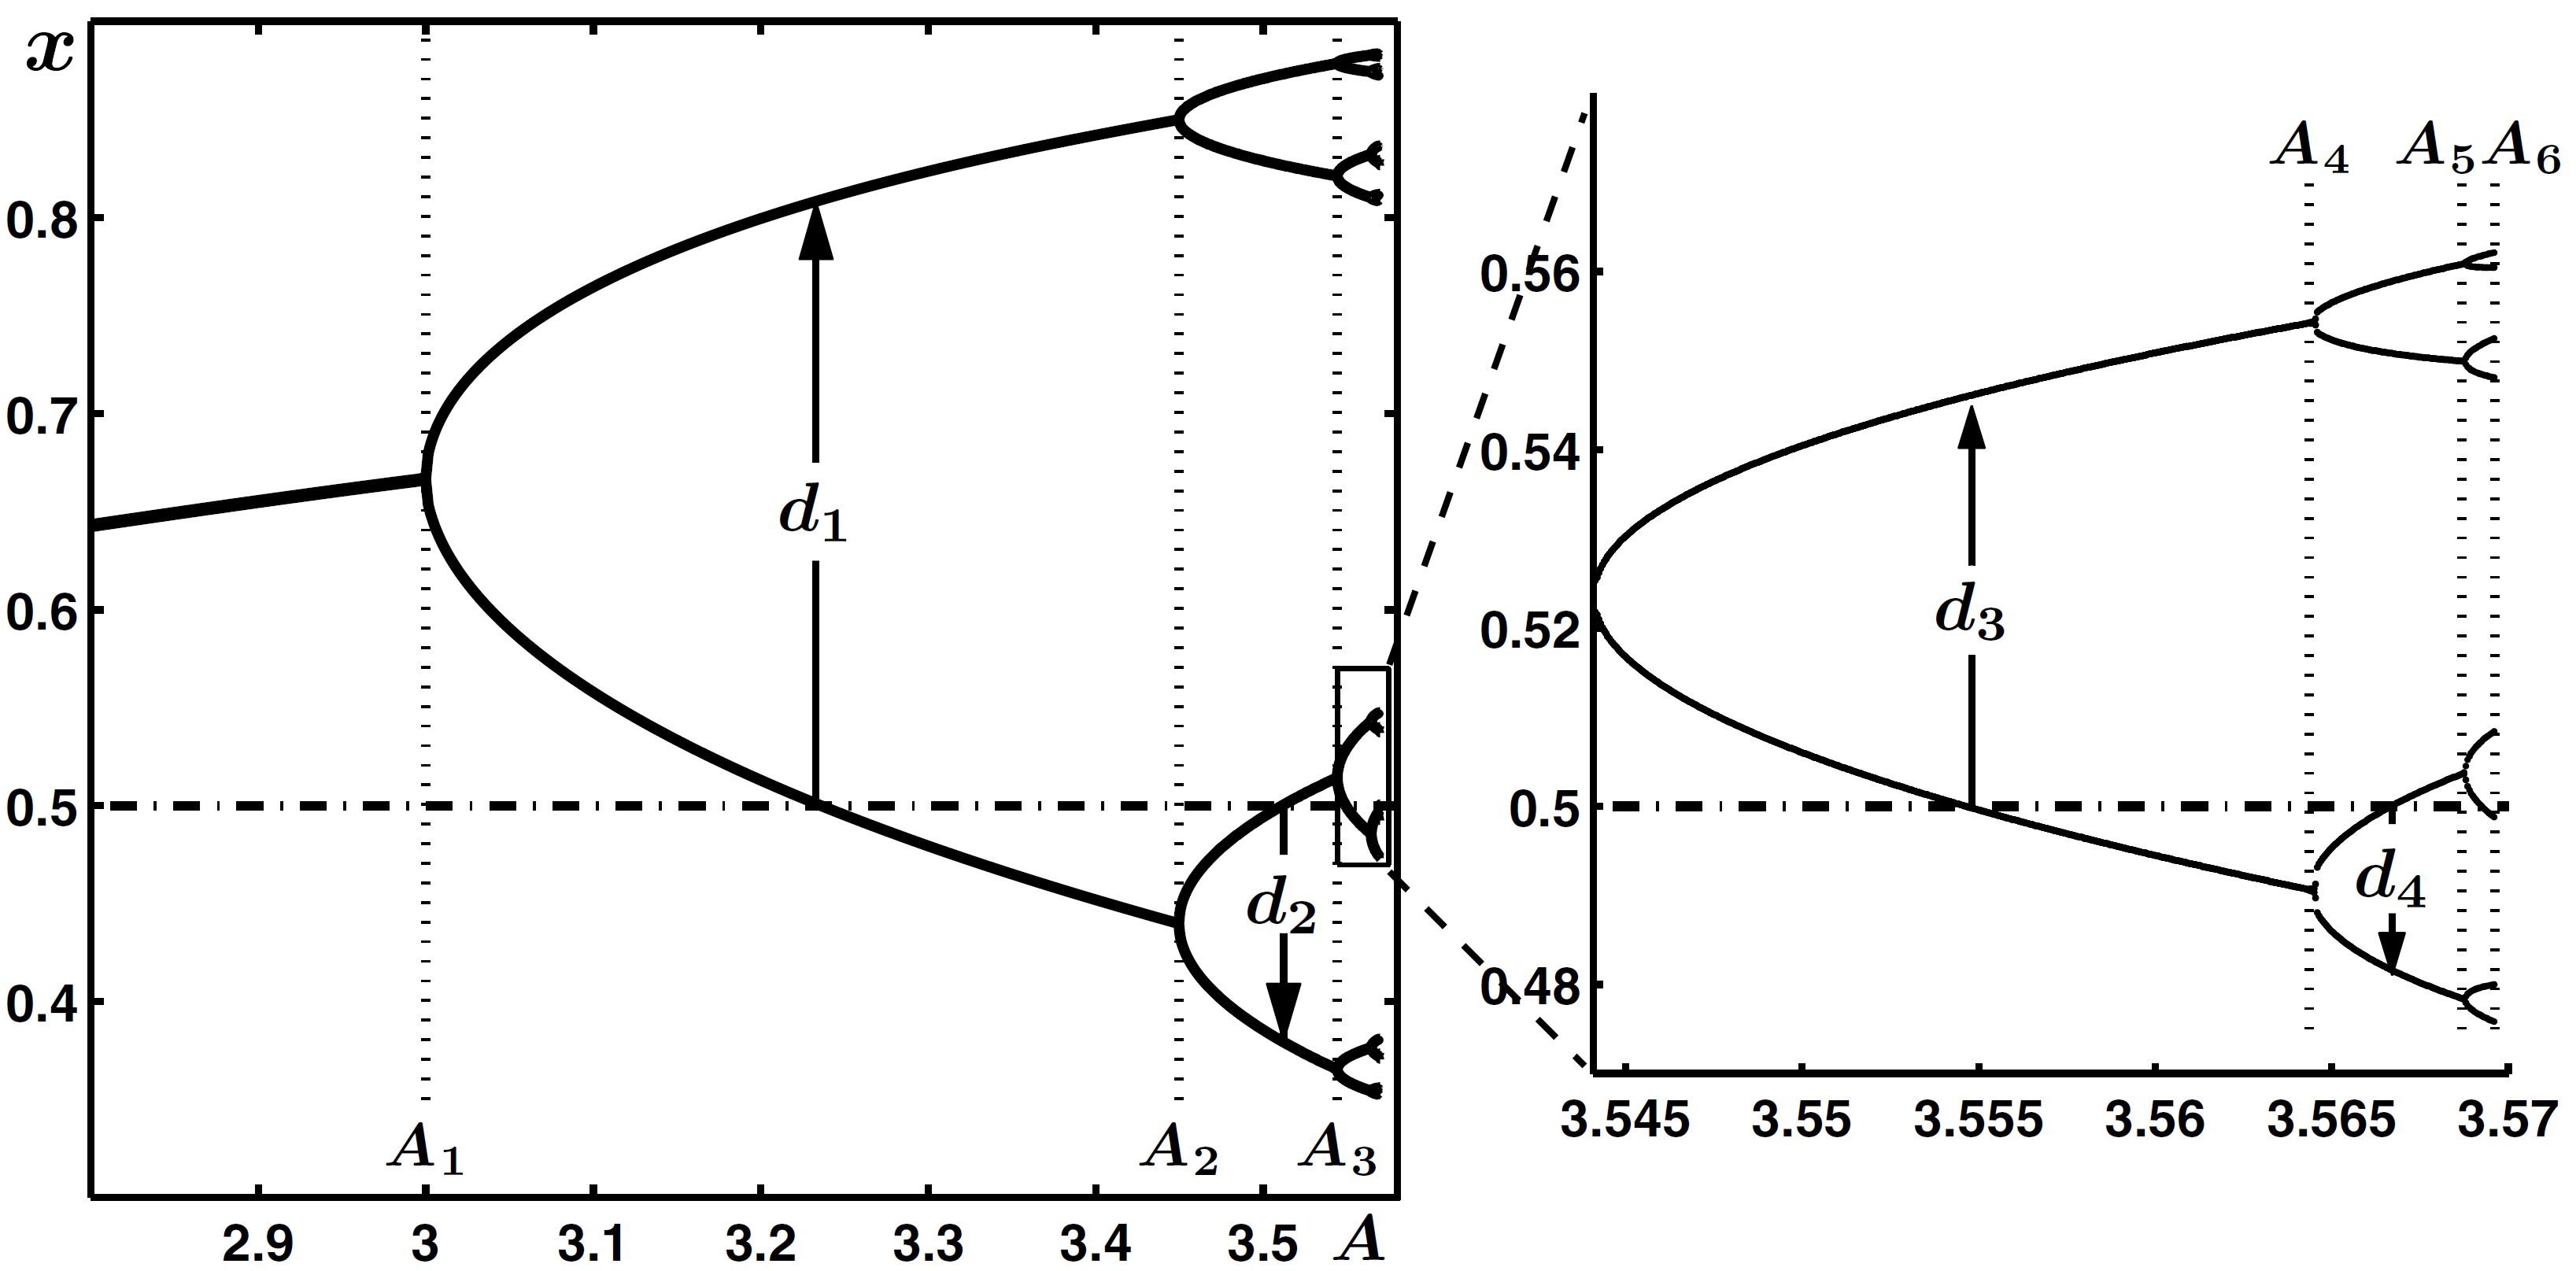
\includegraphics[width=\linewidth]{fca.png}
	\caption{Universal scaling in the horizontal and vertical direction of a period doubling sequence.}
	\label{fig:fca}
\end{wrapfigure}
The number $\delta$, known as the \emph{Feigenbaum constant}, is universal in the sense that it is the same number for a big class of nonlinear maps, differential equations$\ldots$
In addition to the scaling along the parameter axis there is a similar property for the variable $x$ along the vertical axis in a bifurcation diagram.\\
The width of the pitchfork at the \textbf{superstable orbits}\footnote{Superstable orbits are those for which the magnitude of the derivative of an iterate vanishes $|f^{(n)\prime}(x_0)|=0$. For the logistic map $f^\prime(x)=A(1-2x)$ and therefore $x=0.5$ is a superstable orbit. The Lyapunov exponent at such an orbit is $\lambda=-\infty$ (\ref{sec:ledds}).} converges towards another universal constant, known as the Feigenbaum constant $\alpha$.
\begin{equation}
	\alpha=\lim_{n\rightarrow\infty}\frac{d_{n+1}}{d_n}\approx-2.502907875
\end{equation}
As shown in Figure (\ref{fig:fca}) for the first four locations $d_{1-4}$, the pitchfork alternates between above and below the superstable orbit, leading to $d$ values alternating between positive and negative and as a consequence to a negative sign for the constant $\alpha$.